\chapter{Lec 10 - Logical Agents III- First Order Logic}
\section{First Order Logic}
We showed how a knowledge-based agent could represent the world in which it operates and deduce what actions to take. We used propositional logic as our representation language because it sufficed to illustrate the basic concepts of logic and knowledge-based agents. Propositional logic is a \textbf{declarative} language because its semantics is based on a truth relation between sentences and possible worlds. It also has sufficient expressive power to deal with partial information, using disjunction and negation. Propositional logic has a third property that is desirable in representation languages, namely, \textbf{compositionality}. In a compositional language, the meaning of a sentence is a function of the meaning of its parts. However, propositional logic lacks the expressive power to concisely describe an environment with many objects.\newline\newline
We can adopt the foundation of propositional logic—a declarative, compositional semantics that is context-independent and unambiguous—and build a more expressive logic on that foundation, borrowing representational ideas from natural language while avoiding its drawbacks. Whereas propositional logic assumes world contains facts, \textbf{first-order logic} (like natural language) assumes the world contains:
\begin{itemize}
    \item \textbf{Objects}: people, houses, numbers, theories, Ronald McDonald, colors, baseball games, wars, centuries ...

    \item \textbf{Relations}: these can be unary relations or properties such as red, round, bogus, prime, multistoried ..., or more general n-ary relations such as brother of, bigger than, inside, part of, has color, occurred after, owns, comes between, ...

    \item \textbf{Functions}: father of, best friend, third inning of, one more than, beginning of ...
\end{itemize}
Indeed, almost any assertion can be thought of as referring to objects and properties or relations.


\section{Syntax of FOL: Basic elements}
The basic syntactic elements of first-order logic are the symbols that stand for objects, relations, and functions:
\begin{itemize}
    \item \textbf{variable symbols} $x, y, z, ...$
    \item \textbf{constant  symbols} which stand for objects $KingJohn, 2, UCB,...$
    \item \textbf{function symbols}, which stand for functions.
    \item \textbf{predicate symbols}, which stand for relations.
\end{itemize}
Another important part of the syntax are the logical connectives:
\begin{itemize}
    \item \textbf{Propositional connectives}: $\land, \lor, \neg, \Rightarrow$
    \item \textbf{Quantifiers:} $\forall, \exists$
\end{itemize}
\begin{center}
    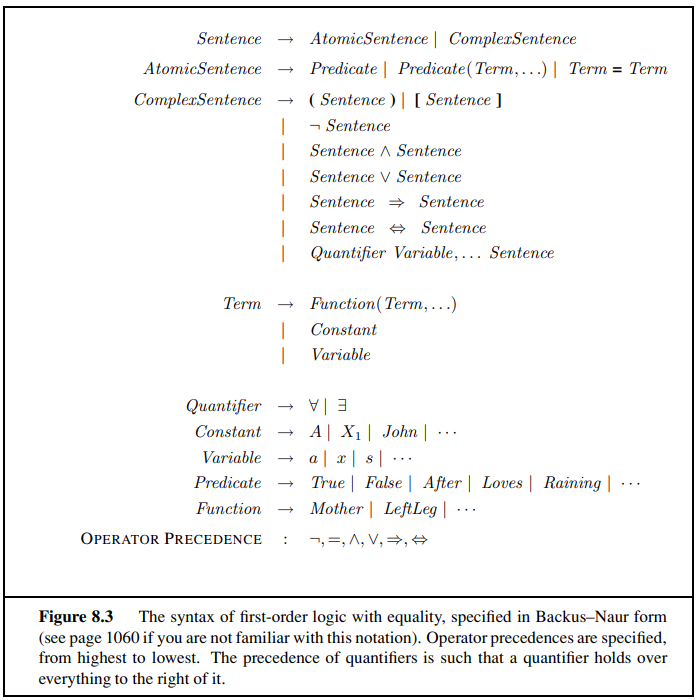
\includegraphics[]{images/FOL.png}
\end{center}

\subsection{Terms}
A \textbf{term} is a logical expression that refers to an object. Constant symbols are therefore terms, but it is not always convenient to have a distinct symbol to name every object. For example, in English we might use the expression “King John’s left leg” rather than giving a name to his leg. This is what function symbols are for: instead of using a constant symbol, we use $LeftLeg(John)$.\newline\newline
In the general case, a complex term is formed by a function symbol followed by a parenthesized list of terms as arguments to the function symbol. A term can also be a constant or a variable.

\subsection{Atomic sentences}
Now that we have both terms for referring to objects and predicate symbols for referring to relations, we can put them together to make \textbf{atomic sentences} that state facts. An \textbf{atomic sentence}  is formed from a predicate symbol optionally followed by a parenthesized list of terms, such as $Brother(Richard, John)$. We can use the equality symbol to signify that two terms refer to the same object. For example, $Father(John) = Henry$. Atomic sentences can have complex terms as arguments. Thus, $Married(Father(Richard), Mother(John))$.

\subsection{Complex sentences}
We can use logical connectives to construct more \textbf{complex sentences}, with the same syntax and semantics as in propositional calculus:
\[\begin{split}
    & \neg Brother (LeftLeg(Richard), John) \\
    & Brother (Richard, John) \land Brother (John, Richard)
\end{split}\]

\section{Models for first-order logic}
The models of a logical language are the formal structures that
constitute the possible worlds under consideration. Each model links the vocabulary of the logical sentences to elements of the possible world, so that the truth of any sentence can be determined. Thus, models for propositional logic link proposition symbols to predefined truth values. Models for first-order logic are much more interesting. First, they have objects in them! The \textbf{domain} of a model is the set of objects or domain elements it contains. The objects in a model may be related in various ways. Formally speaking, a relation is just the set of tuples of objects that are related.
\begin{center}
    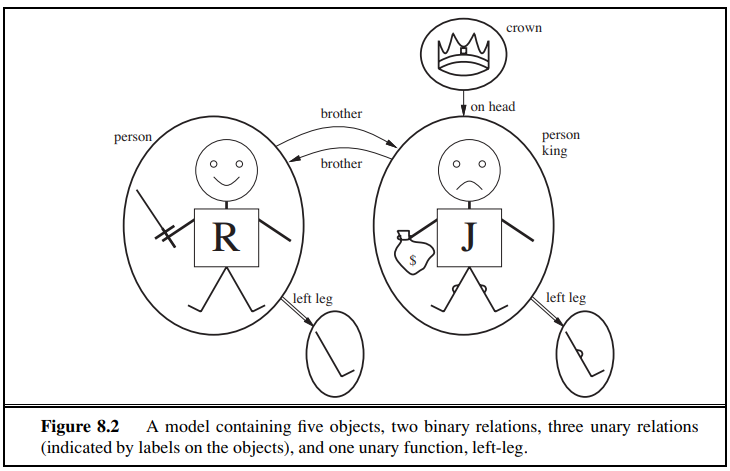
\includegraphics[]{images/FOL model.png}
\end{center}
The figure above shows a model with five objects: Richard the Lionheart, King of England from 1189 to 1199; his younger brother, the evil King John, who ruled from 1199 to 1215; the left legs of Richard and John; and a crown. The crown is on King John’s head, so the “on head” relation contains just one tuple, $<the crown, King John>$. The “brother” and “on head” relations are binary relations, that is, they relate pairs of objects. The model also contains unary relations, or properties: the “person” property is true of both Richard and John; the “king” property is true only of John (presumably because Richard is dead at this point); and the “crown” property is true only of the crown. So far, we have described the elements that populate models for first-order logic. The other essential part of a model is the link between those elements and the vocabulary of the logical sentences.
\newline\newline
As we said previously, constant symbols stand for objects, predicate symbols stand for relations and function symbols stand for functions. Each
predicate and function symbol comes with an \textbf{arity} that fixes the number of arguments. As in propositional logic, every model must provide the information required to determine if any given sentence is true or false. Thus, in addition to its objects, relations, and functions, each model includes an \textbf{interpretation} that specifies exactly which objects, relations and functions are referred to by the constant, predicate, and function symbols. One
possible interpretation for our example is as follows:
\begin{itemize}
    
    
    \item \textbf{Constants}: $Richard$ refers to Richard the Lionheart and $John$ refers to the evil King John.

    \item \textbf{Predicates}: $Brother$ refers to the brotherhood relation, $OnHead$ refers to the “on head” relation that holds between the crown and King John; $Person$, $King$, and $Crown$ refer to the sets of objects that are persons, kings, and crowns.

    \item \textbf{Functions:} $LeftLeg$ refers to the “left leg” function.

\end{itemize}
There are many other possible interpretations, of course. For example, one interpretation maps $Richard$ to the crown and $John$ to King John’s left leg. There are five objects in the model, so there are 25 possible interpretations just for the constant symbols $Richard$ and $John$.\newline\newline
For example, the atomic sentence $Brother(Richard, John)$ states, under the intended interpretation given earlier, that Richard the Lionheart is the
brother of King John. Instead, the atomic sentence \textit{Married(Father (Richard), Mother (John))} states that Richard the Lionheart’s father is married to King John’s mother.\newline\newline
\textit{An atomic sentence is \textbf{true} in a given model if the relation referred to by the predicate symbol holds among the objects referred to by the arguments.}\newline\newline
Here are some complex sentences that are true in the model under our intended interpretation:
\[\begin{split}
    & \neg Brother (LeftLeg(Richard), John)\\
    & Brother (Richard, John) \land Brother (John, Richard)\\
    & King(Richard) \land King(John)\\
    & \neg King(Richard) \Rightarrow King(John) .
\end{split}\]
In summary, a model in first-order logic consists of a set of objects and an interpretation that maps constant symbols to objects, predicate symbols to relations on those objects, and function symbols to functions on those objects.\newline\newline
Because the number of possible models is unbounded, checking entailment by the enumeration of all possible models is not feasible for first-order logic (unlike propositional logic).  Even if the number of objects is restricted, the number of combinations can be very large.


\section{Quantifiers}
Once we have a logic that allows objects, it is only natural to want to express properties of entire collections of objects, instead of enumerating the objects by name. \textbf{Quantifiers} let us do this. First-order logic contains two standard quantifiers, called \textbf{universal} and \textbf{existential}.

\subsection{Universal quantification}
The \textbf{universal quantifier} $\forall$ is of the form $\forall <variables><sentence>$. For example, “All kings are persons,” is written in first-order logic as $\forall\, x \,\, King(x) \Rightarrow Person(x)$. The symbol $x$ is called a \textbf{variable}. By convention, variables are lowercase letters. A variable is a term all by itself, and as such can also serve as the argument of a function.\newline\newline
Intuitively, the sentence $\forall \,x\,\, P$, where $P$ is any logical expression, says that $P$ is true for every object $x$. More precisely, $\forall\, x \,\, P$ is true in a given model if $P$ is true in all possible extended interpretations constructed from the interpretation given in the model, where each extended interpretation specifies a domain element to which $x$ refers. That is, the universally quantified sentence is equivalent to asserting the following five sentences:
\[
\begin{split}
    & \text{Richard the Lionheart is a king} \Rightarrow \text{Richard the Lionheart is a person.}\\
    & \text{King John is a king} \Rightarrow \text{King John is a person.}\\
    & \text{Richard’s left leg is a king} \Rightarrow \text{Richard’s left leg is a person.}\\
    & \text{John’s left leg is a king} \Rightarrow \text{John’s left leg is a person.}\\
    & \text{The crown is a king} \Rightarrow \text{the crown is a person}
\end{split}
\]
Typically, $\Rightarrow$ is the main connective with $\forall$.

\subsection{Existential quantification}
Universal quantification makes statements about every object. Similarly, we can make a statement about some object in the universe without naming it, by using an \textbf{existential quantifier}.\newline\newline
To say, for example, that King John has a crown on his head, we write:
\[\exists\, x\,\,  Crown(x) \land OnHead(x, John)\]
Intuitively, the sentence $\exists\, x\,\, P$ says that $P$ is true for at least one object $x$. More precisely, $\exists \,x \,\, P$ is true in a given model if $P$ is true in at least one extended interpretation that assigns $x$ to a domain element. That is, at least one of the following is true:
\[
\begin{split}
    & \text{Richard the Lionheart is a crown} \land \text{Richard the Lionheart is on John’s head;}\\
    & \text{King John is a crown} \land \text{King John is on John’s head;}\\
    & \text{Richard’s left leg is a crown} \land \text{Richard’s left leg is on John’s head;}\\
    & \text{John’s left leg is a crown} \land \text{John’s left leg is on John’s head;}\\
    & \text{The crown is a crown} \land \text{the crown is on John’s head}
\end{split}
\]
Typically, $\land$ is the main connective with $\exists$.

\subsection{Properties of quantifiers}
We will often want to express more complex sentences using multiple quantifiers:
\begin{itemize}
    \item $\forall x \forall y$ is the same as $\forall y \forall x$;

    \item $\exists x \exists y$ is the same as $\exists y \exists x$;

    \item $\exists x \forall y$ is \textbf{not} the same as $\forall y \exists x$. In fact, $\exists y\forall x \,\,Loves(x, y)$ says that "There is a person who loves everyone in the world". On the other hand, $. \forall\,x (\exists\,y Loves(x, y))$ says that "Everyone in the world is loved by at least one person".

    \item \textbf{Quantifier duality}: each can be expressed using the other:
    \[
    \begin{split}
        \forall\, x \,\, Likes(x,IceCream) & \neg \exists x \,\, \neg Likes(x,IceCream)\\
        \exists \, x \,\, Likes(x, Broccoli) & \neg \forall \, x \,\, \neg Likes(x, Broccoli)
    \end{split}\]
\end{itemize}

\section{Assertions and queries in first-order logic}
Sentences are added to a knowledge base using TELL, exactly as in propositional logic. Such sentences are called assertions. For example, we can assert that John is a king, Richard is a person, and all kings are persons:
\[\begin{split}
    & TELL(KB, King(John)) .\\
    & TELL(KB, Person(Richard)) .\\
    & TELL(KB, \forall \, x King(x) \Rightarrow Person(x)) .
\end{split}\]
We can ask questions of the knowledge base using ASK. For example, $ASK(KB, King(John))$ returns true. Questions asked with ASK are called \textbf{queries} or \textbf{goals}.\newline\newline
If we want to know what value of $x$ makes the sentence true, we will need a different function, ASKVARS, which we call with
\[ASKVARS(KB,Person(x))\]
and which yields a stream of answers. In this case there will be two answers: $\{x/John\}$ and $\{x/Richard\}$. Such an answer is called a \textbf{substitution}.

\section{Inference in First Order Logic}
This section and the next introduce the ideas underlying modern logical inference systems. We begin with some simple inference rules that can be applied to sentences with quantifiers to obtain sentences without quantifiers. These rules lead naturally to the idea that first-order inference can be done by converting the knowledge base to propositional logic and using propositional inference, which we already know how to do. In the future, we will provide an obvious shortcut, leading to inference methods that manipulate first-order sentences directly.

\subsection{Universal Instantiation (UI)}
Let us begin with universal quantifiers. Suppose our knowledge base contains the standard folkloric axiom stating that all greedy kings are evil:
\[\forall \,x \,\, King(x) \land Greedy(x) \Rightarrow Evil(x)\]
Then it seems quite permissible to infer any of the following sentences:
\[
\begin{split}
    & King(John) \land Greedy(John) \Rightarrow Evil(John)\\
    & King(Richard) \land Greedy(Richard) \Rightarrow Evil(Richard)\\
    & King(Father (John)) \land Greedy(Father (John)) \Rightarrow Evil(Father (John))\\
    & .\\
    & .\\
    & .
\end{split}
\]
The rule of \textbf{Universal Instantiation} (\textbf{UI}) says that we can infer any sentence obtained by substituting a ground term (a term without variables) for the variable. Basically, Every instantiation of a universally quantified sentence is entailed by it. To write out the inference rule formally, we use the notion of substitutions introduced previously. Let $Subst(\theta,\alpha)$ denote the result of applying the substitution $\theta$ to the sentence $\alpha$. Then the rule is written as:
\begin{center}
    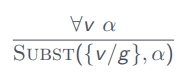
\includegraphics[scale=0.7]{images/UI.png}
\end{center}
for any variable $v$ and ground term $g$. For example, the three sentences given earlier are obtained with the substitutions $\{x/John\}$, $\{x/Richard\}$, and $\{x/Father (John)\}$.

\subsection{Existential Instantiation}
In the rule for \textbf{Existential Instantiation}, the variable is replaced by a single new constant symbol. The formal statement is as follows: for any sentence $\alpha$, variable $v$, and constant symbol $k$ that does not appear elsewhere in the knowledge base, 
\begin{center}
    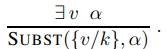
\includegraphics[]{images/EI.png}
\end{center}
For example, from the sentence
\[\exists\, x \,\, Crown(x) \land OnHead(x, John)\]
we can infer the sentence
\[Crown(C1) \land OnHead(C1, John)\]
as long as $C_1$ does not appear elsewhere in the knowledge base. Basically, the existential sentence says there is some object satisfying a condition, and applying the existential instantiation rule just gives a name to that object. Of course, that name must not already belong to another object. $C_1$ is called \textbf{Skolem constant}. Existential Instantiation is a special case of a more general process called \textbf{skolemization}, which we will cover in the future.
\newline\newline
Whereas Universal Instantiation can be applied many times to add new sentences to KB, Existential Instantiation can be applied once, and then the existentially quantified sentence can be discarded. For example, we no longer need $\exists \, x \,\, Kill(x, Victim)$ once we have added the sentence $Kill(Murderer , Victim)$ to KB. Strictly speaking, the new knowledge base is not logically equivalent to the old.

\subsection{Reduction to propositional inference}
Once we have rules for \textit{inferring nonquantified sentences from quantified sentences}, it becomes possible to reduce first-order inference to propositional inference.\newline\newline
The first idea is that, just as an existentially quantified sentence can be replaced by one instantiation, a universally quantified sentence can be replaced by the set of all possible instantiations. For example, suppose our knowledge base contains just the sentences:
\[
\begin{split}
    & \forall \, x \,\, King(x) \land Greedy(x) \Rightarrow Evil(x)\\
    & King(John)\\
    & Greedy(John)\\
    & Brother (Richard, John).
\end{split}
\]
Then we apply UI to the first sentence using all possible ground-term substitutions from the vocabulary of the knowledge base, in this case, $\{x/John\}$ and $\{x/Richard\}$. We obtain:
\[
\begin{split}
    & King(John) \land Greedy(John) \Rightarrow Evil(John)\\
    & King(Richard) \land Greedy(Richard) \Rightarrow Evil(Richard),
\end{split}
\]
and we discard the universally quantified sentence. Now, the knowledge base is essentially propositional if we view the ground atomic sentences, $King (John)$, $Greedy(John)$, and so on, as proposition symbols. Therefore, we can apply any of the complete propositional
algorithms described previously to obtain conclusions such as $Evil(John)$.\newline\newline
However, there is a problem. When the knowledge base includes
a function symbol, the set of possible ground-term substitutions is infinite! For example, if the knowledge base mentions the $Father$ symbol, then infinitely many nested terms such as $Father (Father (Father (John)))$ can be constructed.\newline\newline
Fortunately, there is a famous theorem due to Jacques Herbrand (1930) to the effect that if a sentence is entailed by the original, first-order knowledge base, then there is a proof involving just a finite subset of the propositionalized knowledge base. Since any such subset has a maximum depth of nesting among its ground terms, we can find the subset by first generating all the instantiations with constant symbols ($Richard$ and $John$), then all terms of depth 1 ($Father (Richard)$ and $Father (John)$), then all terms of depth 2, and so on, until we are able to construct a propositional proof of the entailed sentence.\newline\newline
We have sketched an approach to first-order inference via propositionalization that is \textbf{complete}, that is, any entailed sentence can be proved.  On the other hand, we do not know until the
proof is done that the sentence is entailed! What happens when the sentence is not entailed? Alan Turing (1936) and Alonzo Church (1936)
both proved, in rather different ways, that \textit{the question of entailment for first-order logic is semidecidable, that is, algorithms exist that say yes to every entailed sentence, but no algorithm exists that also says no to every nonentailed sentence}.


